\chapter{How Arnoldi Locates Eigenvalues}
The Arnoldi iteration is two things:
\begin{itemize}
    \item The basis of many of the iterative algorithms of NLA 
    \item A techniques for finding eigenvalues of nonhermitian matrices. 
\end{itemize} 

\section{Computing Eigenvalues by the Arnoldi Iteration} 

This is how we compute the eigenvalues: at each iteration, we compute the eigenvalues of $ H_n $ by QR algorithm. Some of these numbers are typically observed to converge rapidly, often geometrically. Suppose $n\ll m$, typically, the Arnoldi iteration will find extreme eigenvalues, which are near the edge of the spectrum of $ A $. 

\section{ A note of Caution: Nonnormality} 
If the answer is highly sensitive to perturbations, you have probably asked the wrong question. We urge anyone faced with nonhermitian eigenvalue computations involving highly sensitive eigenvalues to bear this principle in mind. If you are a numerical analyst, and the problem was given to you by a colleague in science or engineering, do not accept without scrutiny your colleague's assurances that it is truly the eigenvalues that matter physically, even though their condition numbers with respect to perturbations of the matrix entries are $10^4$. 

\section{ Arnoldi and Polynomial Approximation} 
$ \forall x \in \cK_n $, we have 
\[
    x = c_0b+c_1Ab+c_2A^{2} b + \cdots +c_{ n-1 } A^{n-1}b = q(A)b, 
\]
where $ q(z) = c_0 +c_1z +c_2 z^{2} +\cdots + c_{n-1}z^{n-1} $.  One analysis of Arnoldi iteration considers 
\[
    P^{n} = \{\text{ monic polynomials of degree }n\} .
\]

We have the following problem. 


%────────────────────────────────────────
\begin{example}
[Arnoldi/Lanczos Approximation Problem]
\label{eg: Arnoldi/Lanczos Approximation Problem}
\begin{equation}
\label{eq: Arnoldi approx problem}
        \arg\min_{p^{n}\in P^{n}}  \|p^{n}(A)b\|. 
\end{equation}
\end{example}
%────────────────────────────────────────

The Arnoldi iteration has the remarkable property that it solves this problem exactly. 


%────────────────────────────────────────
\begin{theorem}
\label{thm: prop of Arnoldi iteration}
As long as the Arnoldi iteration does not break down (i.e., $ K_n $ is of full rank $ n $), \eqref{eq: Arnoldi approx problem} has a unique solution $ p^{n} $, the characteristic polynomial of $ H_n $.  
\end{theorem}
%────────────────────────────────────────
%────────────────────────────────────────
\begin{proof}[Proof sketch]
Note that $ p(A)b = A^{n}b - Q_n y$ for some $ y \in \CC^n $.  Hence, we are projecting $ A^{n}b $ to $ \cK_n $ and we must have $ p^n(A)b\perp \cK_n \Leftrightarrow Q_n^*  p^{n}(A)b= 0 $. Now we replace $ A $ with its decomposition $ QHQ^*  $. At step $ n $, we know that 
\[
    Q = [Q_{n} U], \quad H = \begin{bmatrix}[] 
        H_n &  X_1 \\
        X_2 &  X_3 \\
    \end{bmatrix}. 
\]
Here $ (X_2)_{ij} = 0$ except $ (X_2)_{11} $.  Plug in this into our condition, we get 
\[
    Q_n^*  Q p^{n}(H) Q^*  b = Q_n^* Q p^n (H) \|b\|e_1 = I_{n,m} p^{n}(H)\|b\|e_1 = 0. 
\]
Hence, the first $ n $ entries of the first column of $ p^n(H) $ are all zero. Note that these are also the first $ n $ entries of the first column of $ p^n(H_n) $. Because we can check $ H\cdot H^m $ to verify this. Since the characteristic polynomial of $ H_n $ satisfies the condition, this is one solution. If we we have another $ p^{n} $, we subtract them and get a polynomial $ q $ of degree $ n-1 $ and $q(A)b\perp \cK_n$. Note that $ q(A)b $ is also in $ \cK_n $. Hence, $ q(A)b = 0 $, violating the assumption that $ \cK_n $ is of full rank. 

\end{proof}
%────────────────────────────────────────

\section{Invariance Properties}
Since the family $ P^{n} $ of monic polynomials is invariant with respect to translations $ z\mapsto z+\alpha $, the Arnoldi iteration is also translation-invariant. 


%────────────────────────────────────────
\begin{theorem}
[Invariance of Arnoldi iteration]
Let the Arnoldi iteration be applied to a matrix $A \in \mathbb{C}^{m \times m}$ as described above.

Translation-invariance. If $A$ is changed to $A+\sigma I$ for some $\sigma \in \mathbb{C}$, and $b$ is left unchanged, the Ritz values $\left\{\theta_j\right\}$ at each step change to $\left\{\theta_j+\sigma\right\}$.

Scale-invariance. If $A$ is changed to $\sigma A$ for some $\sigma \in \mathbb{C}$, and $b$ is left unchanged, the Ritz values $\left\{\theta_j\right\}$ change to $\left\{\sigma \theta_j\right\}$.

Invariance under unitary similarity transformations. If $A$ is changed to $U A U^*$ for some unitary matrix $U$, and $b$ is changed to $U b$, the Ritz values $\left\{\theta_j\right\}$ do not change.

In all three cases the $\mathrm{Ritz}$ vectors, namely the vectors $Q_n y_j$ corresponding to the eigenvectors $y_j$ of $H_n$, do not change under the indicated transformation.
\end{theorem}
%────────────────────────────────────────

every matrix $A$ is unitarily similar to an upper-triangular matrix. Thus the property of invariance under unitary similarity transformations implies that for understanding convergence properties of the Arnoldi iteration, it is enough in principle to consider upper-triangular matrices. 


\section{How Arnoldi Locates Eigenvalues} 
What does polynomial approximation have to do with the eigenvalues of $A$ ? A little thought shows that there is a connection between these two along the following lines. If one's aim is to find a polynomial $p^n$ with the property that $p^n(A)$ is small, an effective means to that end may be to pick $p^n$ to have zeros close to the eigenvalues of $A$.


Consider an extreme case. Suppose that $A$ is diagonalizable and has only $n \ll m$ distinct eigenvalues, hence a minimal polynomial of degree $n$. Then from Theorem~\ref{thm: prop of Arnoldi iteration} it is clear that after $n$ steps, all of these eigenvalues will be found exactly, at least if the vector $b$ contains components in directions associated with every eigenvalue. Thus after $n$ steps, the Arnoldi iteration has computed the minimal polynomial of $A$ exactly.

In practical applications, much the same phenomenon takes place. Now, however, the agreement of Ritz values with eigenvalues is approximate instead of exact, and instead of a minimal polynomial, the result is a "pseudo-minimal polynomial," i.e., a polynomial $p^n$ such that $\left\|p^n(A)\right\|$ is small.


\section{Arnoldi Lemniscates}

%────────────────────────────────────────
\begin{definition}
[Lemniscate]
\label{def: Lemniscate}
Given a polynomial $ p $ and a constant $ C $,  a lemniscate is a curve or collection of curves 
\[
    \{z\in \CC: |p(z)| = C\}.  
\]
If $ p$ is the Arnoldi polynomial and $ C = \frac{\|p^{n}(A)b\|}{\|b\|} $, the curves are called Arnoldi lemniscates. 
\end{definition}
%────────────────────────────────────────

As the iteration number $ n $ increases, components of these lemniscates typically appear which surround the extreme eigenvalues of $ A $ and then shrink rapidly to a point, namely the eigenvalue itself.  

One example is let $ A \in \RR^{100\times 100} $ and $ a_{ij}\sim \cN(0, \frac{1}{100}) $.  We have the eigenvalues are approximately uniformly distributed in the unit disk $ |z|\le 1 $.  Now we set $ a_{11} = 1.5 $. 

%────────────────────────────────────────
\begin{figure}[H]
    \centering
    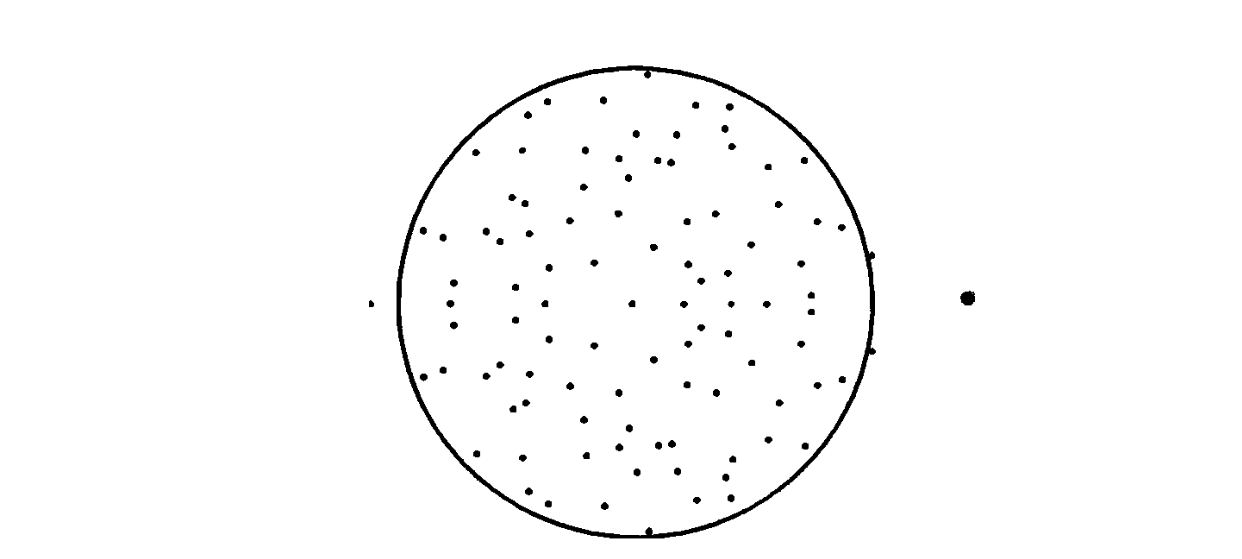
\includegraphics[width=0.6\textwidth]{figures/33-1.png}
    \caption{Eigenvalues of $a 100 \times 100$ matrix $A$, random except in the 1,1 position. The circle is the unit circle in $\mathbb{C}$. The eigenvalues are approximately uniformly distributed in the unit disk except for the outlier $\lambda \approx 1.4852$.}
\end{figure}
%────────────────────────────────────────

%────────────────────────────────────────
\begin{figure}[H]
    \centering
    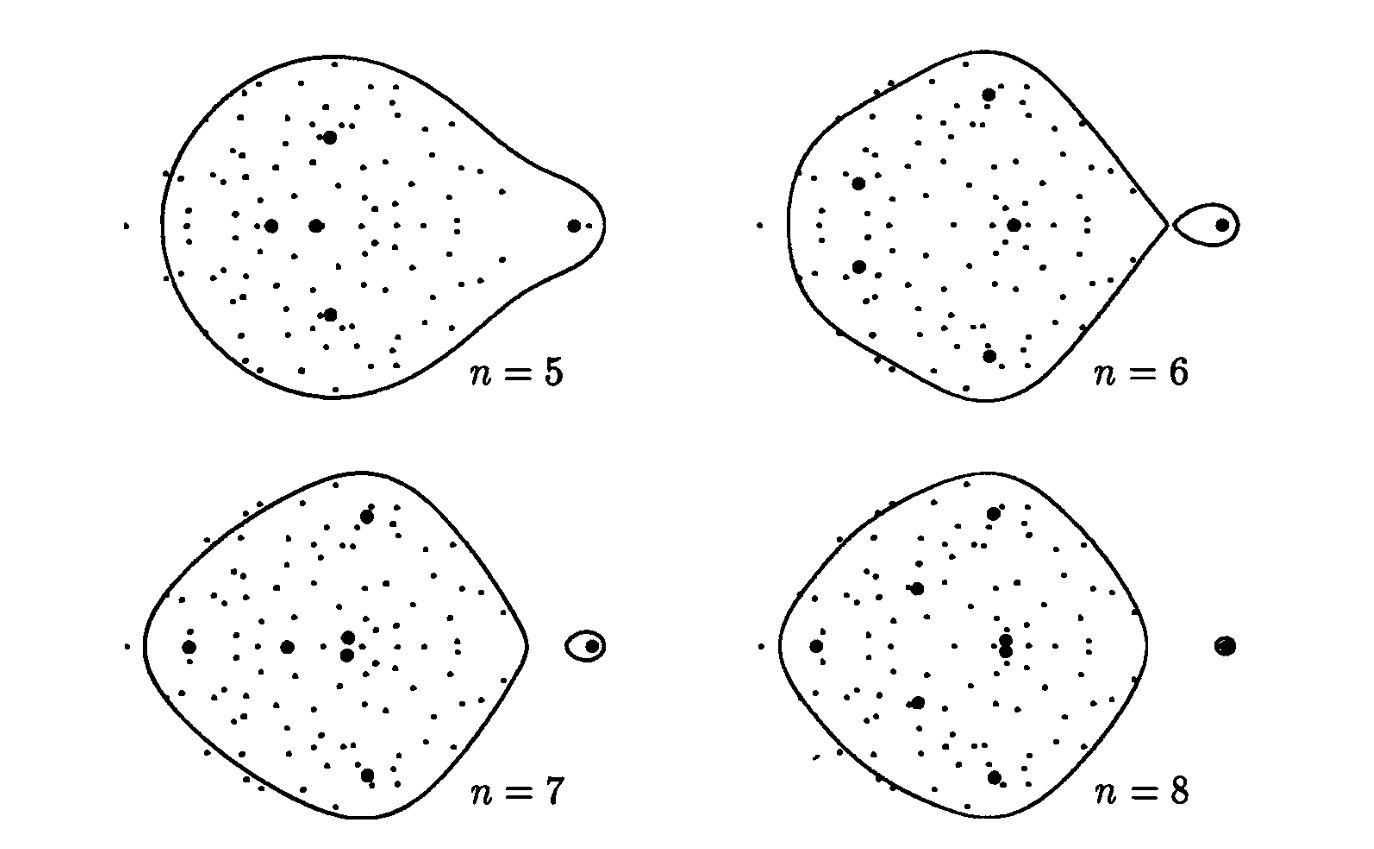
\includegraphics[width=0.6\textwidth]{figures/33-2.png}
    \caption{Arnoldi lemniscates at steps $n=5,6,7,8$ for the same matrix $A$. The small dots are the eigenvalues of $A$, and the large dots are the eigenvalues of $H_n$, i.e., the Ritz values. One component of the Arnoldi lemniscate first "swallows" the outlier eigenvalue, and in subsequent iterations it then shrinks to a point at a geometric rate.}
\end{figure}
%────────────────────────────────────────
 
 \section{Geometric Convergence} 
 Under certain circumstances, the convergence of some of the Arnoldi eigenvalue estimates to eigenvalues of $A$ is geometric. These matters are incompletely understood at present, and we shall not cite theoretical results here. Instead, we shall just take a look at the convergence in the numerical example above, and give a partial explanation.
 
 We still consider the example above and show the following convergence result: 
 %────────────────────────────────────────
 \begin{figure}[H]
    \centering
    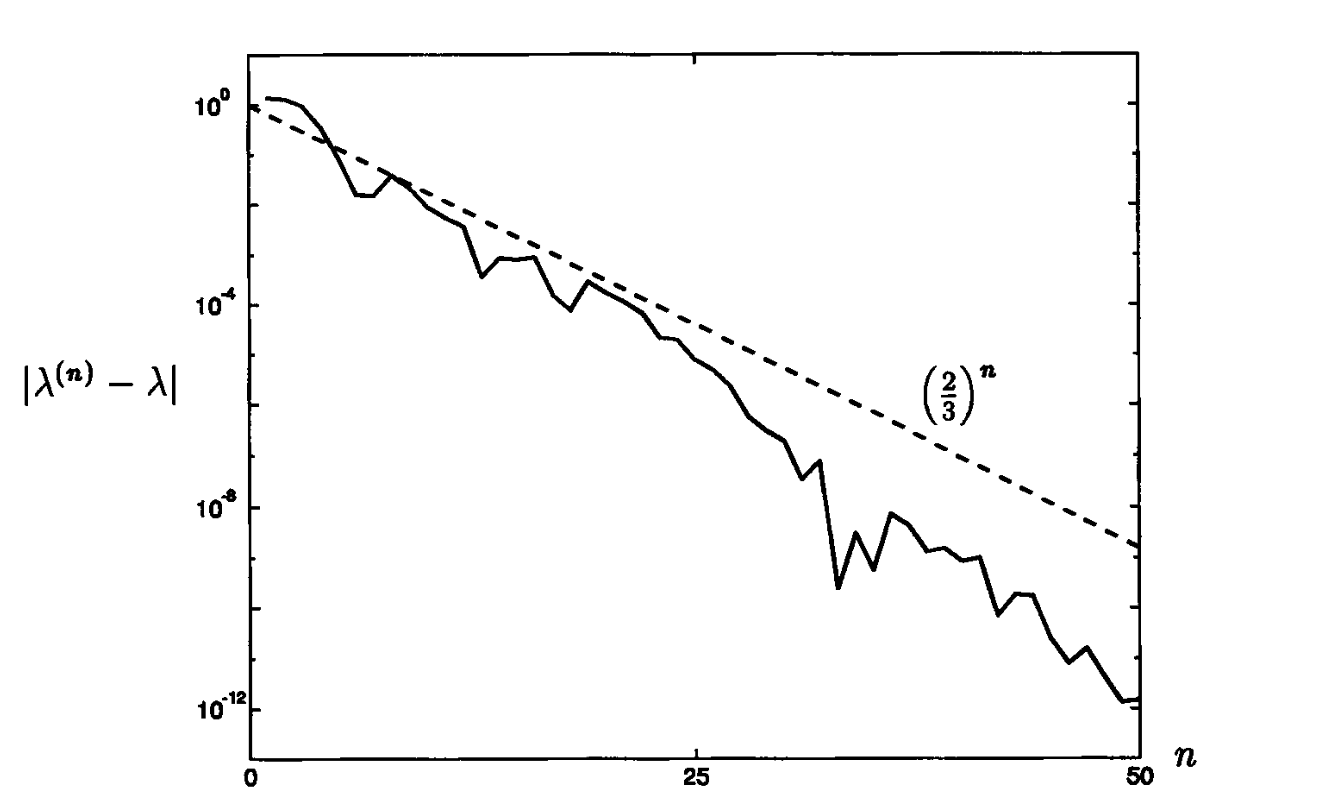
\includegraphics[width=0.8\textwidth]{figures/33-3.png}
    \caption{Convergence of the rightmost Arnoldi eigenvalue estimate.}
 \end{figure}
 %────────────────────────────────────────
 Firstly, we can see that 
 \[
    |\lambda ^{(n)} - \lambda | \approx \left( \frac{2}{3} \right) ^{n}. 
 \]
 An explanation is that we consider the polynomial $ p(z) = z^{n-1}(z-\tilde \lambda ) $ where $ \tilde \lambda  $ is some number close to $ \lambda  $. At each of the eigenvalues of $A$ in the unit disk, $|p(z)|$ is of order 1 or smaller. At $z=\lambda$, however, it has magnitude
 $$
 |p(\lambda)| \approx\left(\frac{3}{2}\right)^n|\tilde{\lambda}-\lambda|
 $$
 (this would be an equality if $\lambda$ were exactly equal to $3 / 2$ ). When $n$ is large, $(3 / 2)^n$ is huge. For this number also to be of order $1,|\tilde{\lambda}-\lambda|$ must be small enough to balance it, that is, of order $(2 / 3)^n$. 

 Another feature is apparent in Figure 34.4. After the initial few dozen steps, the convergence begins to accelerate, a phenomenon common in Krylov subspace iterations. What is happening here is that the iteration is beginning to resolve some of the other outer eigenvalues of $A$, near the unit circle. If the dimension of $A$ had been $m=300$, then the cloud of eigenvalues would have filled the unit disk sufficiently densely that no such acceleration would have been visible in the fifty iterative steps. 